\documentclass[aspectratio=169]{beamer}

\usetheme{default}
\usecolortheme{default}
\usefonttheme{professionalfonts}

\usepackage[T1]{fontenc}
\usepackage{lmodern}
\usepackage{tikz}
\usepackage{booktabs}
\usepackage{array}
\usepackage{tabularx}
\usepackage{graphicx}
\usepackage{listings}
\usetikzlibrary{positioning,arrows.meta,calc,fit,shapes.geometric}

\definecolor{MemphisBlue}{RGB}{26,62,122}
\definecolor{LightBand}{RGB}{244,247,252}
\definecolor{MidBand}{RGB}{229,236,247}
\definecolor{SoftGray}{RGB}{90,96,108}
\definecolor{AccentGreen}{RGB}{61,130,89}
\definecolor{AccentOrange}{RGB}{194,111,46}
\definecolor{AccentRed}{RGB}{168,65,65}

\setbeamertemplate{navigation symbols}{}
\setbeamertemplate{itemize item}{\color{MemphisBlue}$\blacktriangleright$}
\setbeamertemplate{itemize subitem}{\color{MemphisBlue}$\circ$}
\setbeamercolor{title}{fg=MemphisBlue}
\setbeamercolor{frametitle}{fg=MemphisBlue,bg=white}
\setbeamercolor{author in head/foot}{fg=MemphisBlue,bg=white}
\setbeamercolor{date in head/foot}{fg=MemphisBlue,bg=white}
\setbeamerfont{frametitle}{size=\Large,series=\bfseries}
\setbeamerfont{title}{size=\LARGE,series=\bfseries}
\setbeamerfont{subtitle}{size=\large}
\setbeamerfont{normal text}{size=\normalsize}
\setbeamercolor{block body}{bg=LightBand,fg=black}

\setbeamertemplate{footline}{%
  \leavevmode%
  \hbox{%
    \begin{beamercolorbox}[wd=.76\paperwidth,ht=2.6ex,dp=1.2ex,leftskip=1.2em]{author in head/foot}%
      \scriptsize NDNSF-DistributedRepo: Design and Mechanisms
    \end{beamercolorbox}%
    \begin{beamercolorbox}[wd=.24\paperwidth,ht=2.6ex,dp=1.2ex,rightskip=1.2em plus1fil]{date in head/foot}%
      \scriptsize \insertframenumber/\inserttotalframenumber
    \end{beamercolorbox}%
  }%
}

\newcommand{\bluebox}[1]{%
  \begin{beamercolorbox}[rounded=true,shadow=false,sep=0.65em,wd=\linewidth]{block body}
  #1
  \end{beamercolorbox}
}

\newcommand{\evidence}[1]{%
  \vfill\par\noindent
  {\color{SoftGray}\tiny Evidence: #1}\par
}

\tikzset{
  flow/.style={-{Stealth[length=2.2mm]},thick,draw=MemphisBlue},
  dashflow/.style={-{Stealth[length=2.2mm]},thick,dashed,draw=AccentOrange},
  box/.style={draw=MemphisBlue,fill=LightBand,rounded corners=2pt,
    minimum height=0.72cm,align=center,font=\scriptsize},
  strongbox/.style={draw=MemphisBlue,fill=MidBand,rounded corners=2pt,
    minimum height=0.78cm,align=center,font=\scriptsize\bfseries},
  greenbox/.style={draw=AccentGreen,fill=AccentGreen!10,rounded corners=2pt,
    minimum height=0.72cm,align=center,font=\scriptsize},
  orangebox/.style={draw=AccentOrange,fill=AccentOrange!10,rounded corners=2pt,
    minimum height=0.72cm,align=center,font=\scriptsize},
  redbox/.style={draw=AccentRed,fill=AccentRed!8,rounded corners=2pt,
    minimum height=0.72cm,align=center,font=\scriptsize}
}

\title{NDNSF-DistributedRepo}
\subtitle{A High-Availability NDN-Native Repository for NDNSF Applications}
\author{Tianxing Ma}
\institute{Department of Computer Science\\University of Memphis}
\date{July 2026}

\begin{document}

\begin{frame}[plain]
  \titlepage
\end{frame}

\begin{frame}{Why a Service-Aware Repository?}
\footnotesize
\begin{columns}[T]
\begin{column}{0.47\textwidth}
\textbf{NDNSF invocation is intentionally short-lived}

\vspace{0.5em}
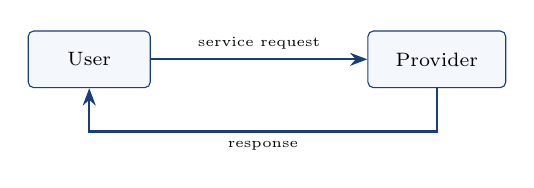
\begin{tikzpicture}[node distance=0.55cm]
  \node[box,minimum width=1.55cm] (user) {User};
  \node[box,right=2.75cm of user,minimum width=1.75cm] (provider) {Provider};
  \draw[flow] (user) -- node[above,font=\tiny] {service request} (provider);
  \draw[flow] (provider.south) -- ++(0,-0.55cm) -|
    node[below,pos=0.25,font=\tiny] {response} (user.south);
\end{tikzpicture}

\vspace{0.8em}
The request/ACK/selection/response path should not carry every large or durable object inline.
\end{column}
\begin{column}{0.49\textwidth}
\textbf{Applications need named data products that outlive one call}

\vspace{0.35em}
\begin{itemize}
  \item Model and runtime artifacts
  \item UAV recordings, telemetry, and mission logs
  \item Intermediate data, configurations, and workflow records
\end{itemize}

\vspace{0.35em}
\bluebox{
\textbf{Repo goal:} keep these objects named, discoverable, replicated, and retrievable without teaching the framework their application meaning.
}
\end{column}
\end{columns}
\evidence{NDNSF-DistributedRepo/README.md, overview and Application Integration Status}
\end{frame}

\begin{frame}{Responsibility Boundary}
\footnotesize
\begin{center}
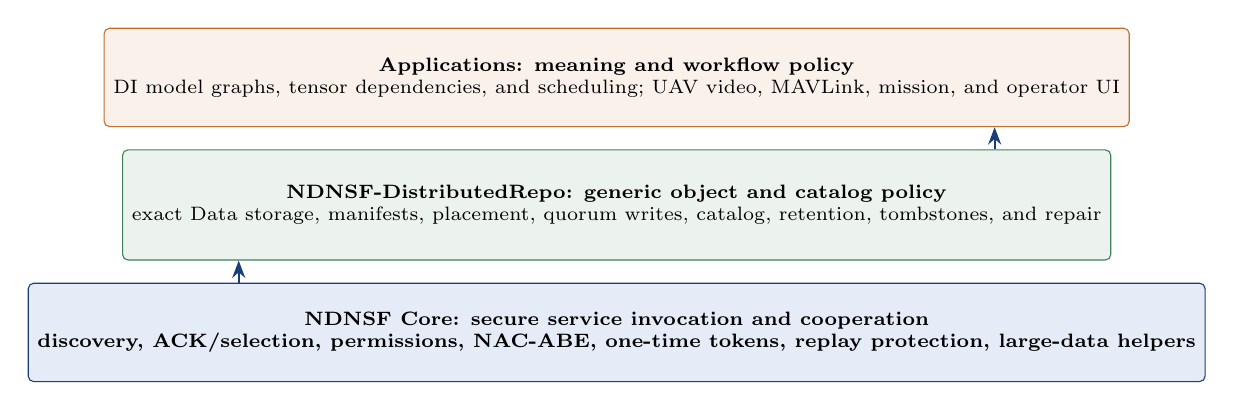
\begin{tikzpicture}[node distance=0.28cm]
  \node[orangebox,minimum width=12.3cm,minimum height=1.25cm] (apps) {
    \textbf{Applications: meaning and workflow policy}\\
    DI model graphs, tensor dependencies, and scheduling; UAV video, MAVLink, mission, and operator UI
  };
  \node[greenbox,below=of apps,minimum width=12.3cm,minimum height=1.4cm] (repo) {
    \textbf{NDNSF-DistributedRepo: generic object and catalog policy}\\
    exact Data storage, manifests, placement, quorum writes, catalog, retention, tombstones, and repair
  };
  \node[strongbox,below=of repo,minimum width=12.3cm,minimum height=1.25cm] (core) {
    \textbf{NDNSF Core: secure service invocation and cooperation}\\
    discovery, ACK/selection, permissions, NAC-ABE, one-time tokens, replay protection, large-data helpers
  };
  \draw[flow] ([xshift=-4.8cm]core.north) -- ([xshift=-4.8cm]repo.south);
  \draw[flow] ([xshift=4.8cm]repo.north) -- ([xshift=4.8cm]apps.south);
\end{tikzpicture}
\end{center}

\vspace{0.25em}
\bluebox{
The repo is reusable because it understands \textbf{named objects and lifecycle metadata}, not AI models, videos, or missions.
}
\evidence{NDNSF-DistributedRepo/README.md, In-App Repo Plan and Application Integration Status}
\end{frame}

\begin{frame}{Layered Architecture}
\footnotesize
\begin{columns}[T]
\begin{column}{0.58\textwidth}
\begin{center}
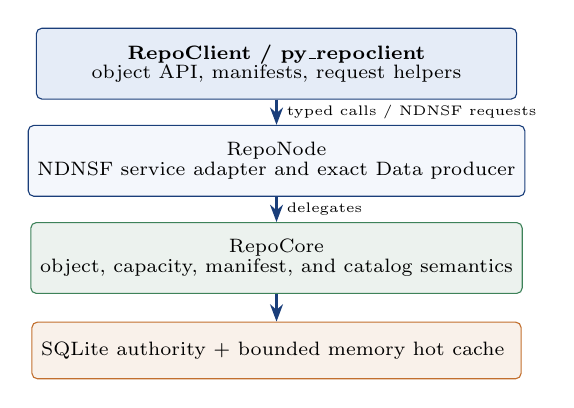
\begin{tikzpicture}[node distance=0.32cm]
  \node[strongbox,minimum width=6.1cm,minimum height=0.9cm] (client) {
    RepoClient / py\_repoclient\\[-0.1em]
    \normalfont object API, manifests, request helpers
  };
  \node[box,below=of client,minimum width=6.1cm,minimum height=0.9cm] (node) {
    RepoNode\\[-0.1em]
    \normalfont NDNSF service adapter and exact Data producer
  };
  \node[greenbox,below=of node,minimum width=6.1cm,minimum height=0.9cm] (core) {
    RepoCore\\[-0.1em]
    \normalfont object, capacity, manifest, and catalog semantics
  };
  \node[orangebox,below=0.35cm of core,minimum width=5.8cm] (backend) {
    SQLite authority + bounded memory hot cache
  };
  \draw[flow] (client) -- node[right,font=\tiny] {typed calls / NDNSF requests} (node);
  \draw[flow] (node) -- node[right,font=\tiny] {delegates} (core);
  \draw[flow] (core) -- (backend);
\end{tikzpicture}
\end{center}
\end{column}
\begin{column}{0.39\textwidth}
\textbf{One durable state model, two exposure paths}
\begin{itemize}
  \item Remote services use the normal NDNSF network path.
  \item Trusted same-process callers use \texttt{LocalServiceRegistry}.
  \item Both paths invoke the same RepoCore semantics.
  \item Memory accelerates hot reads; SQLite remains authoritative.
\end{itemize}

\vspace{0.3em}
\bluebox{Neither local invocation nor the hot cache creates a second object model or a memory-only durability mode.}
\end{column}
\end{columns}
\evidence{RepoClient.hpp, RepoNode.hpp, RepoCore.hpp, RepoTypes.hpp}
\end{frame}

\begin{frame}{Two Deployment Roles}
\footnotesize
\begin{columns}[T]
\begin{column}{0.48\textwidth}
\textbf{In-App Repo}
\begin{itemize}
  \item Embedded in a trusted application process
  \item SQLite-backed local objects and bounded hot cache
  \item Useful for artifacts, recordings, and intermediates
  \item Exposed through local services, remote services, or both
\end{itemize}

\vspace{0.25em}
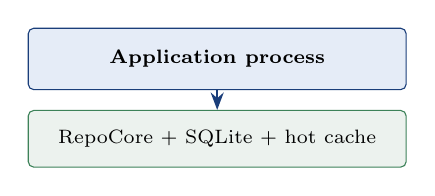
\begin{tikzpicture}[node distance=0.25cm]
  \node[strongbox,minimum width=4.8cm] (app) {Application process};
  \node[greenbox,below=of app,minimum width=4.8cm] (inapp) {RepoCore + SQLite + hot cache};
  \draw[flow] (app) -- (inapp);
\end{tikzpicture}
\end{column}
\begin{column}{0.48\textwidth}
\textbf{Persistent Repo}
\begin{itemize}
  \item Independent NDNSF provider process
  \item Durable backup, shared catalog, and recovery role
  \item Normally accepts backup replicas
  \item SQLite backend remains fetchable after restart
\end{itemize}

\vspace{0.25em}
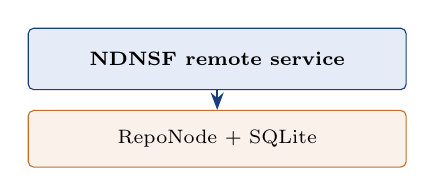
\begin{tikzpicture}[node distance=0.25cm]
  \node[strongbox,minimum width=4.8cm] (remote) {NDNSF remote service};
  \node[orangebox,below=of remote,minimum width=4.8cm] (persistent) {RepoNode + SQLite};
  \draw[flow] (remote) -- (persistent);
\end{tikzpicture}
\end{column}
\end{columns}

\vspace{0.1em}
\bluebox{Both roles use SQLite authority; deployment changes exposure and placement, not object semantics.}
\evidence{README: In-App and Persistent Repo Modes; DistributedRepoNodeApp.cpp}
\end{frame}

\begin{frame}{Two Namespace Planes}
\footnotesize
\begin{center}
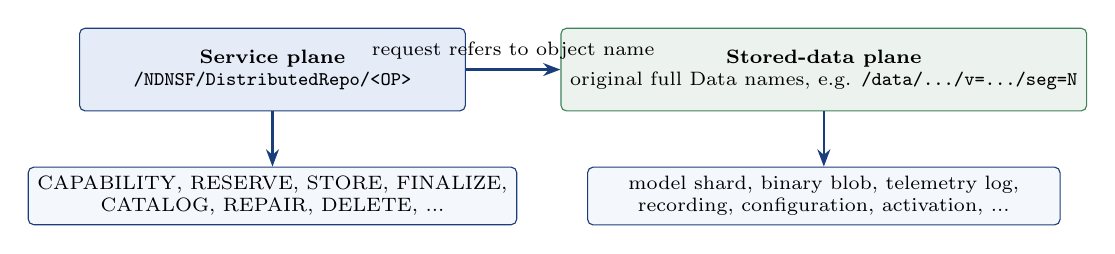
\begin{tikzpicture}[node distance=0.75cm]
  \node[strongbox,minimum width=4.9cm,minimum height=1.05cm] (service) {
    \textbf{Service plane}\\
    \texttt{/NDNSF/DistributedRepo/<OP>}
  };
  \node[greenbox,right=1.2cm of service,minimum width=6.0cm,minimum height=1.05cm] (data) {
    \textbf{Stored-data plane}\\
    original full Data names, e.g. \texttt{/data/.../v=.../seg=N}
  };
  \draw[flow] (service) -- node[above,font=\scriptsize] {request refers to object name} (data);

  \node[box,below=0.7cm of service,minimum width=4.9cm] (ops) {
    CAPABILITY, RESERVE, STORE, FINALIZE,\\CATALOG, REPAIR, DELETE, ...
  };
  \node[box,below=0.7cm of data,minimum width=6.0cm] (objects) {
    model shard, binary blob, telemetry log,\\recording, configuration, activation, ...
  };
  \draw[flow] (service) -- (ops);
  \draw[flow] (data) -- (objects);
\end{tikzpicture}
\end{center}

\vspace{0.45em}
\begin{itemize}
  \item The shared service prefix tells NDNSF \emph{what operation to invoke}.
  \item The original publisher-owned full name tells NDN \emph{which exact Data packet is stored}; Repo does not rename or re-sign it.
\end{itemize}
\evidence{README: Namespace and Trust Schema Design}
\end{frame}

\begin{frame}{Logical Object and Data Reference}
\footnotesize
\begin{columns}[T]
\begin{column}{0.55\textwidth}
\textbf{RepoObjectManifest}

\vspace{0.25em}
\begin{tabularx}{\linewidth}{@{}>{\bfseries}l X@{}}
\toprule
Field & Purpose \\
\midrule
objectName & Stable application object name \\
objectType & Generic application classification \\
sha256, size & End-to-end integrity metadata \\
segmentCount & Logical object layout \\
replicas & Desired factor and confirmed repo nodes \\
consistency & ONE, QUORUM, or ALL receipt threshold \\
lifecycle & STAGED, COMMITTED, or deleted \\
policyEpoch & Placement-policy version \\
\bottomrule
\end{tabularx}
\end{column}
\begin{column}{0.41\textwidth}
\textbf{RepoDataReference}

\vspace{0.25em}
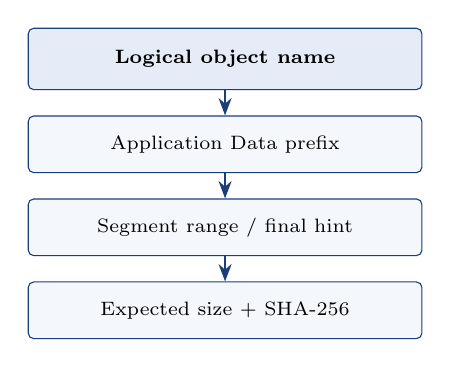
\begin{tikzpicture}[node distance=0.32cm]
  \node[strongbox,minimum width=5.0cm] (obj) {Logical object name};
  \node[box,below=of obj,minimum width=5.0cm] (prefix) {Application Data prefix};
  \node[box,below=of prefix,minimum width=5.0cm] (range) {Segment range / final hint};
  \node[box,below=of range,minimum width=5.0cm] (integrity) {Expected size + SHA-256};
  \draw[flow] (obj) -- (prefix);
  \draw[flow] (prefix) -- (range);
  \draw[flow] (range) -- (integrity);
\end{tikzpicture}

\vspace{0.3em}
The reference lets a repo pull application-published signed Data without putting the large payload in the service request.
\end{column}
\end{columns}
\evidence{RepoTypes.hpp: RepoObjectManifest and RepoDataReference}
\end{frame}

\begin{frame}{INSERT: Store App-Owned Segmented Data}
\footnotesize
\begin{center}
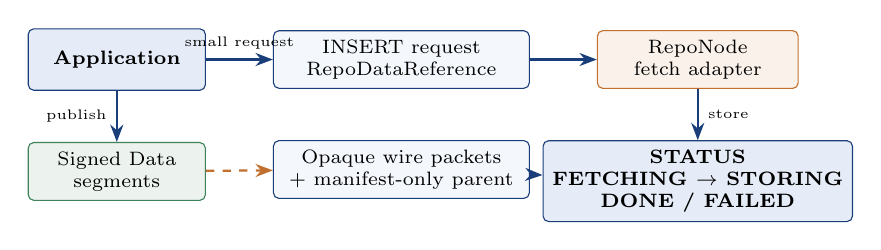
\begin{tikzpicture}[node distance=0.55cm]
  \node[strongbox,minimum width=2.25cm] (app) {Application};
  \node[box,right=0.85cm of app,minimum width=3.25cm] (request) {INSERT request\\RepoDataReference};
  \node[orangebox,right=0.85cm of request,minimum width=2.55cm] (repo) {RepoNode\\fetch adapter};
  \draw[flow] (app) -- node[above,font=\tiny] {small request} (request);
  \draw[flow] (request) -- (repo);

  \node[greenbox,below=0.65cm of app,minimum width=2.25cm] (data) {Signed Data\\segments};
  \node[box,below=0.65cm of request,minimum width=3.25cm] (stored) {Opaque wire packets\\+ manifest-only parent};
  \node[strongbox,below=0.65cm of repo,minimum width=2.55cm] (status) {STATUS\\FETCHING $\to$ STORING\\DONE / FAILED};
  \draw[flow] (app) -- node[left,font=\tiny] {publish} (data);
  \draw[dashflow] (data) -- (stored);
  \draw[flow] (repo) -- node[right,font=\tiny] {store} (status);
  \draw[flow] (stored) -- (status);
\end{tikzpicture}
\end{center}

\vspace{0.15em}
\bluebox{The repo stores wire packets as opaque bytes. It does not decrypt, reinterpret, or re-authorize the application payload.}
\evidence{RepoNode::handleInsert; README: App-Owned Segmented Data References}
\end{frame}

\begin{frame}{Payload APIs Are Adapters, Not Another Data Model}
\footnotesize
\begin{columns}[T]
\begin{column}{0.60\textwidth}
\begin{center}
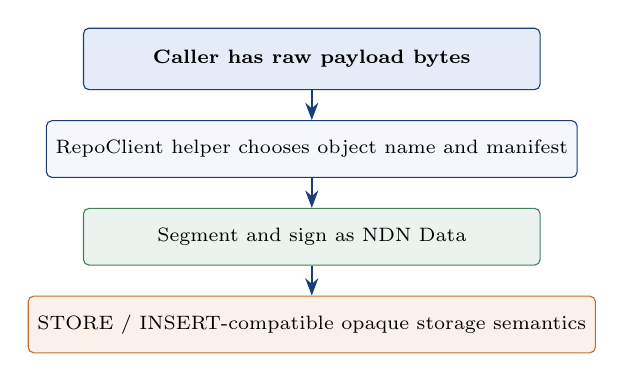
\begin{tikzpicture}[node distance=0.38cm]
  \node[strongbox,minimum width=5.8cm] (raw) {Caller has raw payload bytes};
  \node[box,below=of raw,minimum width=5.8cm] (client) {RepoClient helper chooses object name and manifest};
  \node[greenbox,below=of client,minimum width=5.8cm] (segment) {Segment and sign as NDN Data};
  \node[orangebox,below=of segment,minimum width=5.8cm] (store) {STORE / INSERT-compatible opaque storage semantics};
  \draw[flow] (raw) -- (client);
  \draw[flow] (client) -- (segment);
  \draw[flow] (segment) -- (store);
\end{tikzpicture}
\end{center}
\end{column}
\begin{column}{0.36\textwidth}
\textbf{Why keep the adapters?}
\begin{itemize}
  \item Convenient for existing callers and tests
  \item Same logical object and manifest API
  \item Same opaque backend and catalog semantics
\end{itemize}

\vspace{0.35em}
\bluebox{Large files use named segmented Data. Continuous video publication remains a stream problem, not a repo object problem.}
\end{column}
\end{columns}
\evidence{RepoClient::insertPayload, putSegmented, getObject; NDNSF large-data boundary}
\end{frame}

\begin{frame}{Fetch Exact Data, Fail Over by Replica}
\footnotesize
\begin{center}
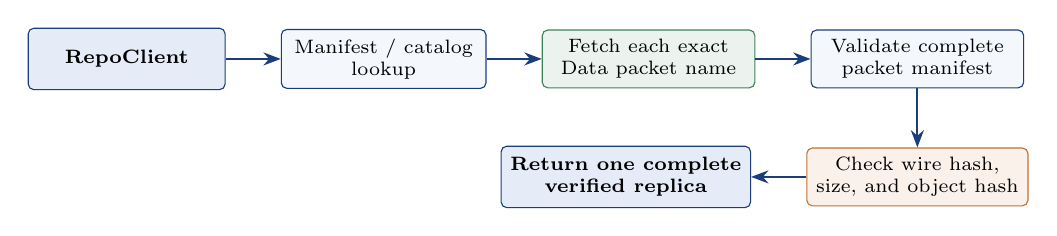
\begin{tikzpicture}[node distance=0.7cm]
  \node[strongbox,minimum width=2.5cm] (client) {RepoClient};
  \node[box,right=of client,minimum width=2.6cm] (lookup) {Manifest / catalog\\lookup};
  \node[greenbox,right=of lookup,minimum width=2.7cm] (fetch) {Fetch each exact\\Data packet name};
  \node[box,right=of fetch,minimum width=2.7cm] (assemble) {Validate complete\\packet manifest};
  \draw[flow] (client) -- (lookup);
  \draw[flow] (lookup) -- (fetch);
  \draw[flow] (fetch) -- (assemble);

  \node[orangebox,below=0.75cm of assemble,minimum width=2.7cm] (verify) {Check wire hash,\\size, and object hash};
  \node[strongbox,left=0.7cm of verify,minimum width=2.7cm] (app) {Return one complete\\verified replica};
  \draw[flow] (assemble) -- (verify);
  \draw[flow] (verify) -- (app);
\end{tikzpicture}
\end{center}

\vspace{0.45em}
\begin{columns}[T]
\begin{column}{0.48\textwidth}
\textbf{Repo responsibility:} reject malformed/partial packet sets and retry the whole object at another replica.
\end{column}
\begin{column}{0.48\textwidth}
\textbf{Application responsibility:} apply domain trust and decrypt or interpret the verified Data.
\end{column}
\end{columns}
\evidence{RepoClient::fetchSignedPackets; exact-packet and replica-failover regressions}
\end{frame}

\begin{frame}{Capability-Driven Replica Placement}
\footnotesize
\begin{center}
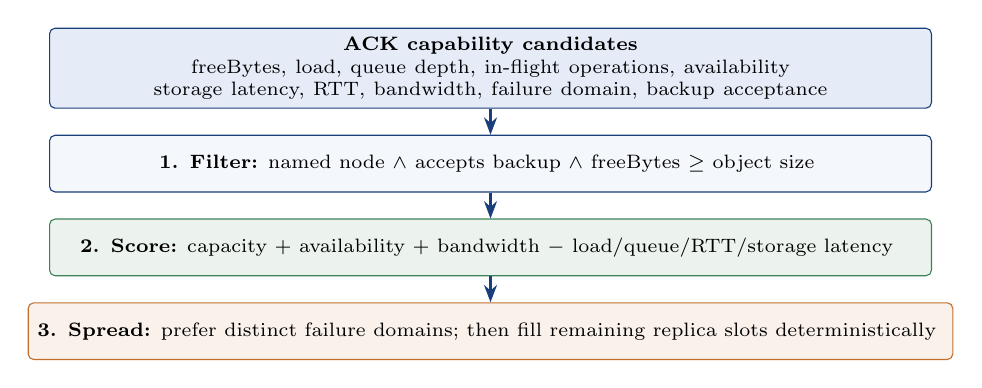
\begin{tikzpicture}[node distance=0.33cm]
  \node[strongbox,minimum width=11.2cm,text width=10.8cm] (acks) {
    ACK capability candidates\\
    \normalfont freeBytes, load, queue depth, in-flight operations, availability\\
    storage latency, RTT, bandwidth, failure domain, backup acceptance
  };
  \node[box,below=of acks,minimum width=11.2cm] (filter) {
    \textbf{1. Filter:} named node $\land$ accepts backup $\land$ freeBytes $\ge$ object size
  };
  \node[greenbox,below=of filter,minimum width=11.2cm] (score) {
    \textbf{2. Score:} capacity + availability + bandwidth $-$ load/queue/RTT/storage latency
  };
  \node[orangebox,below=of score,minimum width=11.2cm] (spread) {
    \textbf{3. Spread:} prefer distinct failure domains; then fill remaining replica slots deterministically
  };
  \draw[flow] (acks) -- (filter);
  \draw[flow] (filter) -- (score);
  \draw[flow] (score) -- (spread);
\end{tikzpicture}
\end{center}

\vspace{0.3em}
\bluebox{Placement uses live provider capability hints, then reserves capacity before sending replicated writes.}
\evidence{RepoTypes.cpp: scoreCandidate and selectReplicas; py\_repoclient capability helpers}
\end{frame}

\begin{frame}{Targeted Parallel Write and Quorum Finalization}
\footnotesize
\begin{center}
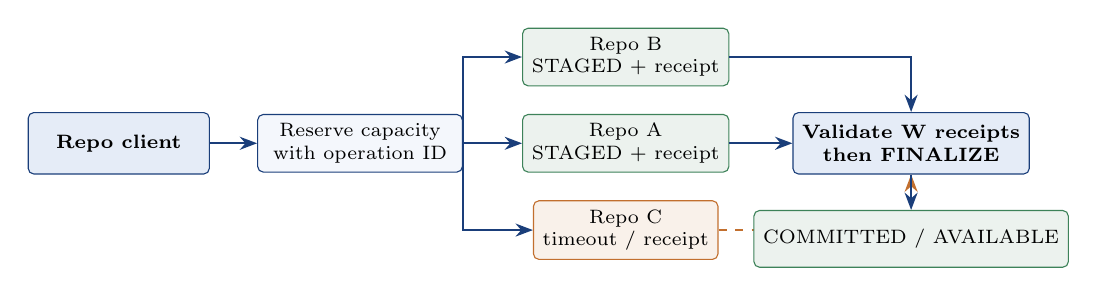
\begin{tikzpicture}[node distance=0.38cm]
  \node[strongbox,minimum width=2.3cm] (user) {Repo client};
  \node[box,right=0.6cm of user,minimum width=2.6cm] (reserve) {Reserve capacity\\with operation ID};
  \node[greenbox,right=0.75cm of reserve,minimum width=2.3cm] (a) {Repo A\\STAGED + receipt};
  \node[greenbox,above=0.35cm of a,minimum width=2.3cm] (b) {Repo B\\STAGED + receipt};
  \node[orangebox,below=0.35cm of a,minimum width=2.3cm] (c) {Repo C\\timeout / receipt};
  \draw[flow] (user) -- (reserve);
  \draw[flow] (reserve) -- (a);
  \draw[flow] (reserve.east) |- (b.west);
  \draw[flow] (reserve.east) |- (c.west);

  \node[strongbox,right=0.8cm of a,minimum width=2.65cm] (commit) {Validate W receipts\\then FINALIZE};
  \draw[flow] (a) -- (commit);
  \draw[flow] (b.east) -| (commit.north);
  \draw[dashflow] (c.east) -| (commit.south);
  \node[greenbox,below=0.45cm of commit,minimum width=2.65cm] (visible) {COMMITTED / AVAILABLE};
  \draw[flow] (commit) -- (visible);
\end{tikzpicture}
\end{center}

\vspace{0.15em}
\begin{columns}[T]
\begin{column}{0.48\textwidth}
\begin{itemize}
  \item RF is desired placement; W is required durable receipts.
  \item ONE, QUORUM, and ALL keep different failure/latency tradeoffs.
\end{itemize}
\end{column}
\begin{column}{0.48\textwidth}
\begin{itemize}
  \item Known replicas use secure Targeted calls in parallel.
  \item Below-quorum STAGED data is invisible to reads and repair.
\end{itemize}
\end{column}
\end{columns}
\bluebox{Targeted reduces control rounds; authorization, one-time tokens, replay protection, and receipt validation remain active.}
\evidence{Specs 078, 079, and 081; Targeted RF=3/W=QUORUM MiniNDN campaigns}
\end{frame}

\begin{frame}{The Catalog Is Object-Level Metadata}
\footnotesize
\begin{columns}[T]
\begin{column}{0.55\textwidth}
\begin{center}
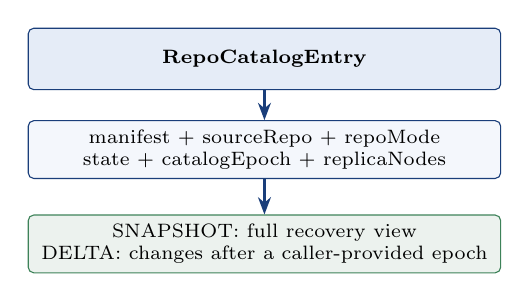
\begin{tikzpicture}[node distance=0.38cm]
  \node[strongbox,minimum width=6.0cm] (entry) {RepoCatalogEntry};
  \node[box,below=of entry,minimum width=6.0cm] (fields) {
    manifest + sourceRepo + repoMode\\state + catalogEpoch + replicaNodes
  };
  \node[greenbox,below=0.45cm of fields,minimum width=6.0cm] (views) {
    SNAPSHOT: full recovery view\\DELTA: changes after a caller-provided epoch
  };
  \draw[flow] (entry) -- (fields);
  \draw[flow] (fields) -- (views);
\end{tikzpicture}
\end{center}
\end{column}
\begin{column}{0.41\textwidth}
\textbf{Catalog operations}
\begin{itemize}
  \item STATUS: node mode, epoch, object count
  \item LOOKUP: one exact logical object
  \item QUERY: class, type, publisher, tags, state, metadata, time range
\end{itemize}

\vspace{0.25em}
\bluebox{Catalogs exchange one record per logical object, not one record per Data segment.}
\end{column}
\end{columns}
\evidence{RepoCatalogStatus/Entry/Delta; README: Catalog and Replica Discovery}
\end{frame}

\begin{frame}{Decentralized Catalog Synchronization}
\footnotesize
\begin{columns}[T]
\begin{column}{0.48\textwidth}
\textbf{Object-level anti-entropy}
\begin{center}
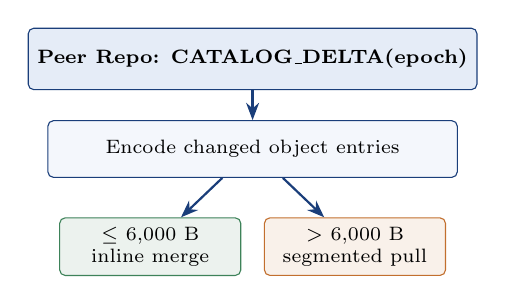
\begin{tikzpicture}[node distance=0.38cm]
  \node[strongbox,minimum width=5.2cm] (peer) {Peer Repo: CATALOG\_DELTA(epoch)};
  \node[box,below=of peer,minimum width=5.2cm] (choose) {Encode changed object entries};
  \node[greenbox,below=0.5cm of choose,xshift=-1.3cm,minimum width=2.3cm] (inline) {$\leq$ 6,000 B\\inline merge};
  \node[orangebox,below=0.5cm of choose,xshift=1.3cm,minimum width=2.3cm] (pull) {$>$ 6,000 B\\segmented pull};
  \draw[flow] (peer) -- (choose);
  \draw[flow] (choose) -- (inline);
  \draw[flow] (choose) -- (pull);
\end{tikzpicture}
\end{center}
\end{column}
\begin{column}{0.48\textwidth}
\textbf{Large-delta integrity path}
\begin{enumerate}
  \item Source publishes signed segmented Data under an exact versioned name.
  \item One protected request binds name, schema, bytes, entries, and SHA-256.
  \item Target fetches the complete object and validates it before merge.
  \item Pull failure falls back to bounded inline batches.
\end{enumerate}
\end{column}
\end{columns}

\vspace{0.3em}
\bluebox{Measured recovered-sidecar path: six large pulls + two inline merges, 33 segments, zero fallback; merge time 5.200 s $\to$ 3.039 s.}
\evidence{Spec 083; catalog\_sync.py; CATALOG\_MERGE\_PULL MiniNDN treatment}
\end{frame}

\begin{frame}{Deletion Uses Tombstones, Not Silence}
\footnotesize
\begin{center}
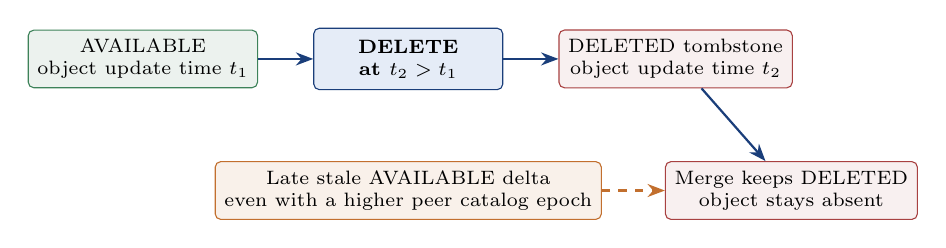
\begin{tikzpicture}[node distance=0.7cm]
  \node[greenbox,minimum width=2.8cm] (available) {AVAILABLE\\object update time $t_1$};
  \node[strongbox,right=of available,minimum width=2.4cm] (delete) {DELETE\\at $t_2 > t_1$};
  \node[redbox,right=of delete,minimum width=2.8cm] (dead) {DELETED tombstone\\object update time $t_2$};
  \draw[flow] (available) -- (delete);
  \draw[flow] (delete) -- (dead);

  \node[orangebox,below=0.9cm of delete,minimum width=4.0cm] (stale) {Late stale AVAILABLE delta\\even with a higher peer catalog epoch};
  \node[redbox,right=0.8cm of stale,minimum width=3.2cm] (shadow) {Merge keeps DELETED\\object stays absent};
  \draw[dashflow] (stale) -- (shadow);
  \draw[flow] (dead) -- (shadow);
\end{tikzpicture}
\end{center}

\vspace{0.5em}
\begin{itemize}
  \item Catalog sequence orders peer changes; object update time and delete semantics resolve object conflicts.
  \item Keeping the tombstone prevents an old replica advertisement from resurrecting removed data.
\end{itemize}
\evidence{generic object store tombstone gossip and epoch-conflict MiniNDN regressions}
\end{frame}

\begin{frame}{Retention and Durable Online Repair}
\footnotesize
\begin{columns}[T]
\begin{column}{0.42\textwidth}
\textbf{Lifecycle policy}
\vspace{0.25em}
\begin{tabularx}{\linewidth}{@{}>{\raggedright\arraybackslash\bfseries}p{2.25cm} X@{}}
\toprule
Condition & Catalog outcome \\
\midrule
Expired & \textcolor{AccentRed}{EXPIRED}; no repair \\
Live + under target & Create repair job \\
Otherwise & Healthy \\
\bottomrule
\end{tabularx}

\vspace{0.35em}
\bluebox{Repair never uses STAGED, deleted, expired, conflicting, or hash-mismatched data as a source.}
\end{column}
\begin{column}{0.54\textwidth}
\textbf{Durable repair job}
\begin{enumerate}
  \item Scan creates idempotent jobs from catalog state.
  \item Risk, priority, age, and replica deficit order claims.
  \item Leased workers fetch exact Data; target verifies and stores.
  \item Success completes; failure backs off.
\end{enumerate}
\end{column}
\end{columns}
\vspace{0.3em}
\bluebox{Sidecar runs repair outside handlers; durable leases and backlog survive restart.}
\evidence{Specs 080--082; durable repair and phase telemetry}
\end{frame}

\begin{frame}{Measured Provider Failure and Recovery}
\footnotesize
\begin{center}
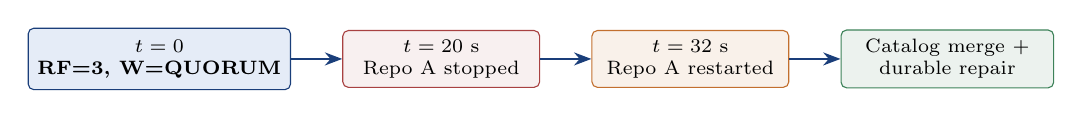
\begin{tikzpicture}[node distance=0.35cm]
  \node[strongbox,minimum width=2.5cm] (start) {$t=0$\\RF=3, W=QUORUM};
  \node[redbox,right=0.65cm of start,minimum width=2.5cm] (fail) {$t=20$ s\\Repo A stopped};
  \node[orangebox,right=0.65cm of fail,minimum width=2.5cm] (restart) {$t=32$ s\\Repo A restarted};
  \node[greenbox,right=0.65cm of restart,minimum width=2.7cm] (repair) {Catalog merge +\\durable repair};
  \draw[flow] (start) -- (fail);
  \draw[flow] (fail) -- (restart);
  \draw[flow] (restart) -- (repair);
\end{tikzpicture}
\end{center}

\vspace{0.4em}
\begin{tabularx}{\linewidth}{@{}>{\bfseries}p{3.6cm} *{3}{>{\centering\arraybackslash}X}@{}}
\toprule
Matched 60 s campaign & Requests & Outage repair & Request p95 \\
\midrule
Quorum during failure & 19/19 post-failure & later repairable & 1,649.912 ms \\
Repair fast path & 30/30 & 4/4 & 1,814.117 ms \\
Catalog segmented pull & 30/30 & 4/4 & 1,779.222 ms \\
\bottomrule
\end{tabularx}

\vspace{0.4em}
\bluebox{Latest fixed treatment: receipt floor W=2, zero invalid repair events, first repair 9.033 s after restart. This is diagnostic evidence, not a production SLO.}
\evidence{Specs 079, 082, and 083 canonical MiniNDN summaries; seed 78004}
\end{frame}

\begin{frame}{Security and Trust Boundaries}
\footnotesize
\begin{center}
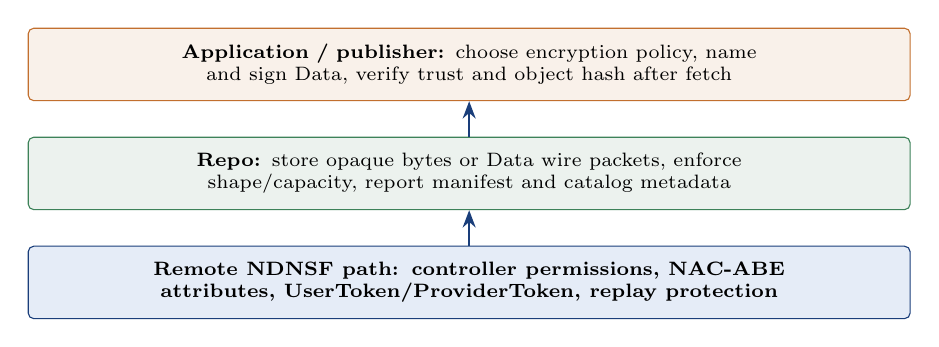
\begin{tikzpicture}[node distance=0.45cm]
  \node[orangebox,minimum width=11.2cm,text width=10.8cm,minimum height=0.92cm] (app) {
    \textbf{Application / publisher:} choose encryption policy, name and sign Data, verify trust and object hash after fetch
  };
  \node[greenbox,below=of app,minimum width=11.2cm,text width=10.8cm,minimum height=0.92cm] (repo) {
    \textbf{Repo:} store opaque bytes or Data wire packets, enforce shape/capacity, report manifest and catalog metadata
  };
  \node[strongbox,below=of repo,minimum width=11.2cm,text width=10.8cm,minimum height=0.92cm] (ndnsf) {
    \textbf{Remote NDNSF path:} controller permissions, NAC-ABE attributes, UserToken/ProviderToken, replay protection
  };
  \draw[flow] (ndnsf) -- (repo);
  \draw[flow] (repo) -- (app);
\end{tikzpicture}
\end{center}

\vspace{0.35em}
\begin{columns}[T]
\begin{column}{0.48\textwidth}
\textbf{Trust schema:} object Data names stay under the publisher identity; child certificates remain under parent namespaces.
\end{column}
\begin{column}{0.48\textwidth}
\textbf{Local path:} trusted same-process composition only; it is never remotely selectable and never weakens remote authorization.
\end{column}
\end{columns}
\evidence{README: Namespace and Trust Schema Design; RepoStoreBackend contract; NDNSF security invariants}
\end{frame}

\begin{frame}{One Generic Repo, Different Applications}
\footnotesize
\begin{center}
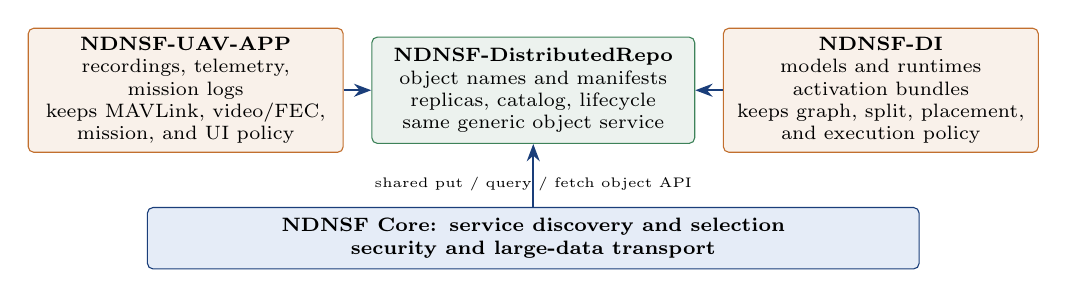
\begin{tikzpicture}[node distance=0.35cm]
  \node[orangebox,minimum width=4.0cm,text width=3.7cm,minimum height=1.35cm] (uav) {
    \textbf{NDNSF-UAV-APP}\\
    recordings, telemetry,\\mission logs\\
    \normalfont keeps MAVLink, video/FEC,\\mission, and UI policy
  };
  \node[greenbox,right=of uav,minimum width=4.1cm,text width=3.8cm,minimum height=1.35cm] (repo) {
    \textbf{NDNSF-DistributedRepo}\\
    object names and manifests\\
    replicas, catalog, lifecycle\\
    \normalfont same generic object service
  };
  \node[orangebox,right=of repo,minimum width=4.0cm,text width=3.7cm,minimum height=1.35cm] (di) {
    \textbf{NDNSF-DI}\\
    models and runtimes\\
    activation bundles\\
    \normalfont keeps graph, split, placement,\\and execution policy
  };
  \draw[flow] (uav) -- (repo);
  \draw[flow] (di) -- (repo);

  \node[strongbox,below=0.8cm of repo,minimum width=9.8cm,text width=9.4cm] (core) {
    NDNSF Core: service discovery and selection\\security and large-data transport
  };
  \node[font=\tiny,above=0.08cm of core] {shared put / query / fetch object API};
  \draw[flow] (core) -- (repo);
\end{tikzpicture}
\end{center}

\vspace{0.35em}
\bluebox{The same object/catalog layer is useful across applications precisely because application semantics stay outside it.}
\evidence{README: Application Integration Status; UAV and DI repo call sites}
\end{frame}

\begin{frame}{What Is Validated Today?}
\footnotesize
\begin{columns}[T]
\begin{column}{0.52\textwidth}
\textbf{Implemented and exercised}
\begin{itemize}
  \item SQLite authority + hot cache across restart
  \item Exact signed Data + replica failover
  \item Parallel Targeted writes + quorum finalization
  \item Provider loss/restart + online repair
  \item Tombstones, conflicts, and segmented anti-entropy
\end{itemize}

\vspace{0.25em}
\begin{beamercolorbox}[sep=0.55em,wd=\linewidth]{block body}
\tiny
\texttt{sudo -E PYTHONPATH=... python3}\\
\texttt{Experiments/NDNSF\_DistributedRepo\_}\\
\texttt{Generic\_Minindn.py}
\end{beamercolorbox}
\end{column}
\begin{column}{0.44\textwidth}
\textbf{Remaining production work}
\begin{itemize}
  \item Larger sustained multi-node campaigns
  \item Crash-point/filesystem durability matrix
  \item WAN partition, churn, and rejoin
  \item Monitoring, quotas, and external receipts
\end{itemize}

\vspace{0.35em}
\bluebox{
\textbf{Takeaway:} exact Data stays on the data plane; authenticated control manages placement, lifecycle, and recovery.
}
\end{column}
\end{columns}
\evidence{Specs 073--083; focused C++/Python/security regressions and canonical MiniNDN results}
\end{frame}

\end{document}
